\begin{filecontents*}{references.bib}
@inproceedings{dragos2022angry,
  title={Angry or sad? emotion annotation for extremist content characterisation},
  author={Dragos, Valentina and Battistelli, Delphine and Etienne, Aline and Constable, Yol{\`e}ne},
  booktitle={Proceedings of the Thirteenth Language Resources and Evaluation Conference},
  pages={193--201},
  year={2022}
}

@phdthesis{etienne2023analyse,
  title={Analyse automatique des {\'e}motions dans les textes: contributions th{\'e}oriques et applicatives dans le cadre de l'{\'e}tude de la complexit{\'e} des textes pour enfants},
  author={Etienne, Aline},
  year={2023},
  school={Universit{\'e} de Nanterre-Paris X}
}

@inproceedings{dragos2023comparison,
  title={Comparison of Classification Techniques for Extremism Detection in French Social Media},
  author={Dragos, Valentina and Constable, Yol{\`e}ne},
  booktitle={2023 26th International Conference on Information Fusion (FUSION)},
  pages={1--6},
  year={2023},
  organization={IEEE}
}

@inproceedings{dragos2024exploring,
  title={Exploring the Emotional Dimension of French Online Toxic Content},
  author={Dragos, Valentina and Battistelli, Delphine and Sow, Fatou and Etienne, Aline},
  booktitle={Proceedings of the 2024 Joint International Conference on Computational Linguistics, Language Resources and Evaluation (LREC-COLING 2024)},
  pages={6945--6954},
  year={2024}
}

@inproceedings{Martin_2020,
  title={{CamemBERT}: a Tasty French Language Model},
  author={Martin, Louis and Muller, Benjamin and Ortiz Su{\'a}rez, Pedro Javier and Dupont, Yoann and Romary, Laurent and de la Clergerie, {\'E}ric and Seddah, Djam{\'e} and Sagot, Beno{\^i}t},
  booktitle={Proceedings of the 58th Annual Meeting of the Association for Computational Linguistics},
  publisher={Association for Computational Linguistics},
  pages={7203--7219},
  year={2020},
  doi={10.18653/v1/2020.acl-main.645},
  url={http://dx.doi.org/10.18653/v1/2020.acl-main.645}
}

@misc{etienne2024emotionidentificationfrenchwritten,
  title={Emotion Identification for French in Written Texts: Considering their Modes of Expression as a Step Towards Text Complexity Analysis},
  author={Aline {\'E}tienne and Delphine Battistelli and Gw{\'e}nol{\'e} Lecorv{\'e}},
  year={2024},
  eprint={2405.14385},
  archivePrefix={arXiv},
  primaryClass={cs.CL},
  url={https://arxiv.org/abs/2405.14385}
}

@article{battistelli2025introduction,
  title={Introduction to the Special Issue of the TAL Journal on Abusive Language: Linguistic Resources, Methods and Applications},
  author={Battistelli, Delphine and Benamara, Farah and Patti, Viviana},
  journal={Traitement Automatique des Langues},
  volume={65},
  number={3},
  pages={7--20},
  year={2025}
}

@book{micheli2014,
  author    = {Micheli, Rapha{\"e}l},
  title     = {Les {\'e}motions dans les discours. Mod{\`e}le d'analyse, perspectives empiriques},
  publisher = {De Boeck Sup{\'e}rieur},
  address   = {Louvain-la-Neuve},
  series    = {Champs linguistiques},
  year      = {2014},
  doi       = {10.3917/dbu.mchel.2014.01}
}

@inproceedings{etienne2022,
  author    = {Etienne, Aline and Battistelli, Delphine and Lecorv{\'e}, Gw{\'e}nol{\'e}},
  title     = {A ({P}sycho-){L}inguistically Motivated Scheme for Annotating and Exploring Emotions in a Genre-Diverse Corpus},
  booktitle = {Proceedings of the Thirteenth Language Resources and Evaluation Conference},
  publisher = {European Language Resources Association},
  address   = {Marseille, France},
  month     = jun,
  year      = {2022},
  pages     = {603--612},
  url       = {https://aclanthology.org/2022.lrec-1.64/}
}

@article{battistelli2025,
  author  = {Battistelli, Delphine and {\'E}tienne, Aline},
  title   = {{ModalE}, une ressource lexicale de la modalit{\'e} au prisme des {\'e}motions},
  journal = {Les Carnets du Cediscor},
  number  = {35},
  year    = {2025},
  note    = {Num{\'e}ro : Marqueurs modaux, {\'e}nonciation et argumentation},
  url     = {https://hal.science/hal-05002259/document}
}
\end{filecontents*}

\PassOptionsToPackage{table}{xcolor}
\documentclass{stageOnera}
%%
% Paquets
%

\usepackage[utf8]{inputenc}
\usepackage[T1]{fontenc}
\usepackage{csquotes}
\usepackage{url}
\usepackage{xcolor}
\definecolor{linkblue}{HTML}{2A8FBD}
\usepackage[
  colorlinks=true,
  linkcolor=linkblue,
  citecolor=linkblue,
  urlcolor=linkblue
]{hyperref}
\usepackage[numbers]{natbib}
\usepackage[french]{babel}
\usepackage{booktabs}
\usepackage{amsmath}
\usepackage{placeins}

%%
% Éléments du cartouche de titre
%

%%% Informations sur le stagiaire

%%%% Nom, prénom
\nom{Tsang}
\prenom{Gwendal}


%%%% Centre, département et unité
\departement{Palaiseau -- DTIS/MIDL}


%%% Informations sur le stage

%%%% Titre complet
% (utilier \par pour forcer le retour à la ligne)
\titre{\large\shortstack[c]{Leveraging linguistic annotations to improve\\automatic detection of online content}}

%%%% thématique (ICS, ISL, 3S, RA, ICIHS, PTI,MACS, IAD, COS)
\thematique{ICS}


%%%% Encadrant(s) (nom, prénom, département/unité)
% (utilier \par pour forcer le retour à la ligne)
\encadrantOnera{Valentina Dragos}
\formation{M2 TAL}

%%%% NE PAS AJOUTER DE MOT CLEFS

\begin{document}

%% Création du cartouche de titre
\maketitle


%% Contenu
\section*{Objectifs}

L'objectif de ce stage est d'étudier dans quelle mesure les signaux émotionnels peuvent compléter l'analyse de contenus toxiques en ligne, en particulier dans des messages liés au cyberharcèlement adolescent. Le travail porte à la fois sur des ressources lexicales, des annotations linguistiques fines et l'évaluation d'un modèle neuronal existant de détection des émotions.

\section*{Contexte}

Le stage s'inscrit dans les travaux du service MIDL du DTIS sur l'analyse des émotions dans les contenus toxiques en ligne. Le sujet est interdisciplinaire : il croise linguistique de corpus, psycholinguistique des émotions et apprentissage automatique appliqué à la détection de contenus abusifs (\textit{Abusive Language Detection}).

La détection automatique des émotions repose historiquement sur des lexiques émotionnels associant des lemmes à des catégories affectives. Nous avons testé ceux développés par Étienne~\citep{etienne2023analyse}, dont le modèle s'appuie également sur une lemmatisation (Stanza). Nous partageons son constat : les lexiques seuls ne suffisent pas à capter la richesse de l'expression émotionnelle, en particulier dans les messages adolescents (abréviations, graphies non standard, sarcasme).\footnote{Scripts d'extraction et de correspondance lexicale : \href{https://github.com/GwenTsang/ExpressionEmotionnelle}{ExpressionEmotionnelle}.}

Pour dépasser cette limite, le stage a mobilisé deux familles d'approches complémentaires. D'une part, EMOTYC, un classifieur RoBERTa multi-label issu de la chaîne TextToKids~\citep{etienne2024emotionidentificationfrenchwritten}, qui prédit 19~labels (présence d'émotion, mode d'expression, catégorie émotionnelle).\footnote{EMOTYC : \href{https://texttokids.ortolang.fr/}{site officiel}, \href{https://huggingface.co/spaces/GwendalTsang/EMOTYC}{démo}, \href{https://gitlab.huma-num.fr/texttokids/ttkwp3-2025}{dépôt}.} D'autre part, des classifieurs linéaires (TF-IDF + LinearSVC, scikit-learn) testés comme baselines. Ce choix fait écho aux résultats de Dragos et Constable~\citep{dragos2023comparison}, qui observent que SVM + TF-IDF surpasse des modèles neuronaux plus lourds pour la détection d'extrémisme en français. Les résultats comparatifs sont présentés dans les sections suivantes.

J'ai par ailleurs annoté manuellement 781~messages issus de \textit{CyberAgression-Large} pour produire le gold émotionnel \textit{CyberAggAdo}, compatible avec les sorties d'EMOTYC.\footnote{Gold et visualisations : \href{https://github.com/GwenTsang/Eval-EMOTYC/blob/main/golds/CyberAdoAgg_gold_global_total.xlsx}{annotations}, \href{https://emotyc.github.io/}{EMOTYC}, \href{https://gwentsang.github.io/}{portfolio}.}

\begin{figure}[htbp]
  \centering
  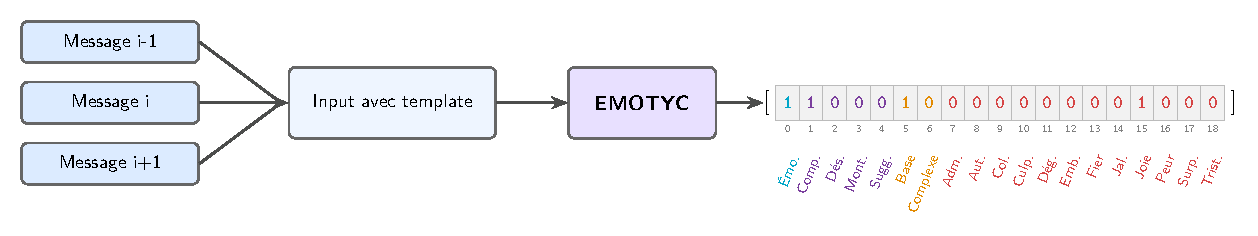
\includegraphics[width=\textwidth,height=0.25\textheight,keepaspectratio]{figures/schema.pdf}
  \caption{Schéma du modèle EMOTYC.}
  \label{fig:schema-emotyc}
\end{figure}

\section*{Objectifs scientifiques}

La modélisation automatique des émotions ne peut toutefois se réduire à l'identification de lexiques émotionnels explicites. Étienne~\citep{etienne2023analyse} distingue quatre modes d'expression, repris ici :

\begin{center}
\footnotesize
\renewcommand{\arraystretch}{1.15}
\begin{tabular}{@{}lp{9.2cm}@{}}
\toprule
Mode & Définition synthétique \\
\midrule
Désignée & émotion nommée par un terme du lexique affectif \\
Comportementale & émotion inférée à partir d'une manifestation physique, discursive ou observable \\
Suggérée & émotion inférée à partir d'une situation ou d'un événement typiquement associé \\
Montrée & émotion portée par la forme même de l'énoncé : syntaxe, ponctuation, typographie ou interjection \\
\bottomrule
\end{tabular}
\end{center}

Les travaux de Dragos et al.~\citep{dragos2022angry}  mettent en évidence la difficulté à localiser des indices émotionnels diffus, implicites ou dépendants du contexte.

Les objectifs scientifiques du stage consistent donc à dépasser une lecture strictement lexicale ou binaire des contenus toxiques, à examiner empiriquement le comportement de modèles d'analyse émotionnelle existants et à déterminer comment leurs sorties peuvent être interprétées pour caractériser plus finement des corpus issus des réseaux sociaux.


\section*{Démarche, déroulement et principaux résultats obtenus}

\subsection{Corpus, ressources et scripts mobilisés}

Le travail a combiné plusieurs types de ressources. D'une part, le corpus \textit{CyberAggAdo} a servi de terrain d'étude principal pour l'analyse de messages de cyberagression adolescente. D'autre part, les résultats sur \textit{TextToKids} ont fourni un point de comparaison avec le domaine d'entraînement d'EMOTYC. Les fichiers de référence, les scripts d'inférence et les sorties d'évaluation sont regroupés dans les dépôts associés au stage.\footnote{Évaluations EMOTYC : \href{https://github.com/GwenTsang/Eval-EMOTYC}{dépôt}, \href{https://github.com/GwenTsang/Eval-EMOTYC/blob/main/results/rapport_performances.md}{rapport}, \href{https://github.com/GwenTsang/Eval-EMOTYC/tree/main/results}{résultats}.}

Un second volet a porté sur les marqueurs émotionnels et leur relation aux émotions et aux modes d'expression. Cette partie s'appuie sur la pipeline \textit{ExpressionEmotionnelle}, sur le corpus \textit{SimpleSitEmo} et sur les rapports statistiques produits à partir des annotations de \textit{CyberAggAdo}.\footnote{Marqueurs et corrélations : \href{https://github.com/GwenTsang/ExpressionEmotionnelle}{dépôt}, \href{https://github.com/GwenTsang/ExpressionEmotionnelle/tree/main/results}{résultats}.}

\subsection{Annotations linguistiques fines et modèle EMOTION}

Le premier axe d'analyse a porté sur le module lexical \textit{EMOTION}, qui associe des lemmes à des catégories émotionnelles.\footnote{Lexique et appariements : \href{https://github.com/GwenTsang/ExpressionEmotionnelle/blob/main/emotions/lexique_emotionnel.tsv}{lexique}, \href{https://github.com/GwenTsang/ExpressionEmotionnelle/tree/main/results/simplesitemo_lexicon_matching}{résultats}.} Cette approche est interprétable et frugale, mais elle reste fragile face aux abréviations, graphies non standard, usages sarcastiques et variations contextuelles des messages adolescents. Un audit local du lexique a aussi relevé une normalisation à harmoniser entre \texttt{degout} et \texttt{dégoût}.

\subsection{Tests du modèle EMOTYC}

Le modèle EMOTYC a été développé dans le cadre du projet ANR TextToKids \citep{etienne2023analyse,etienne2024emotionidentificationfrenchwritten}.\footnote{Modèle et publications : \href{https://huggingface.co/TextToKids/CamemBERT-base-EmoTextToKids}{Hugging Face}, \href{https://texttokids.irisa.fr/publications/}{TextToKids}.} Il s'agit d'un fine-tuning de CamemBERT~\citep{Martin_2020}, entraîné pour une classification multi-label à 19 sorties : présence d'une émotion, mode d'expression, niveau \textit{Base}/\textit{Complexe} et catégorie émotionnelle.

Les évaluations réalisées pendant le stage ont principalement repris la configuration contextuelle utilisée pour le modèle : la phrase cible est fournie avec son contexte immédiat, c'est-à-dire les phrases précédente et suivante. Sur \textit{TextToKids} (27\,911 unités), EMOTYC obtient un Macro-F1 de 0,739 et un Micro-F1 de 0,897. Sur \textit{CyberAggAdo} (781 unités), ces scores chutent à 0,282 et 0,472 respectivement. Plutôt que de reproduire les tableaux détaillés label par label, les deux heatmaps suivantes synthétisent visuellement l'écart de transfert $\Delta_m(\ell) = m_{\text{TextToKids}}(\ell) - m_{\text{CyberAggAdo}}(\ell)$. La couleur encode l'amplitude de $|\Delta|$ : vert clair si les performances sont proches, orange à rouge si l'écart est important.

\begin{table}[htbp]
  \centering
  \small
  \setlength{\tabcolsep}{4pt}
  \begin{tabular}{lrccc}
    \toprule
    \textbf{Label} & \textbf{Cyber} & \textbf{$\Delta F_1$} & \textbf{$\Delta P$} & \textbf{$\Delta R$} \\
    \midrule
    Émo & 398 & \cellcolor[HTML]{C7EA97}\textcolor{black}{+0.27} & \cellcolor[HTML]{D0EB8E}\textcolor{black}{+0.31} & \cellcolor[HTML]{C0EAA2}\textcolor{black}{+0.23} \\
    Base & 363 & \cellcolor[HTML]{E4EC7F}\textcolor{black}{+0.37} & \cellcolor[HTML]{CBEA92}\textcolor{black}{+0.29} & \cellcolor[HTML]{EEDC6F}\textcolor{black}{+0.43} \\
    Montrée & 300 & \cellcolor[HTML]{EEE172}\textcolor{black}{+0.41} & \cellcolor[HTML]{EEDF71}\textcolor{black}{+0.42} & \cellcolor[HTML]{EEE373}\textcolor{black}{+0.41} \\
    Colère & 289 & \cellcolor[HTML]{F0CB66}\textcolor{black}{+0.46} & \cellcolor[HTML]{EEDD6F}\textcolor{black}{+0.42} & \cellcolor[HTML]{F1BA5D}\textcolor{black}{+0.49} \\
    Autre & 62 & \cellcolor[HTML]{E4602C}\textcolor{white}{+0.76} & \cellcolor[HTML]{E25727}\textcolor{white}{+0.78} & \cellcolor[HTML]{E97B39}\textcolor{black}{+0.68} \\
    \bottomrule
  \end{tabular}
  \caption{Heatmap des écarts de performance entre \textit{TextToKids} et \textit{CyberAggAdo} pour les 5~labels les plus représentés dans \textit{CyberAggAdo}. \textit{Cyber} = support dans \textit{CyberAggAdo}. $\Delta > 0$ indique une performance supérieure sur \textit{TextToKids}.}
  \label{tab:heatmap-compact}
\end{table}

\begin{table}[htbp]
  \centering
  \small
  \setlength{\tabcolsep}{4pt}
  \begin{tabular}{lrrccc}
    \toprule
    \textbf{Label} & \textbf{Cyber} & \textbf{TTK} & \textbf{$\Delta F_1$} & \textbf{$\Delta P$} & \textbf{$\Delta R$} \\
    \midrule
    Autre & 62 & 1\,270 & \cellcolor[HTML]{E4602C}\textcolor{white}{+0.76} & \cellcolor[HTML]{E25727}\textcolor{white}{+0.78} & \cellcolor[HTML]{E97B39}\textcolor{black}{+0.68} \\
    Suggérée & 54 & 1\,909 & \cellcolor[HTML]{E5682F}\textcolor{black}{+0.73} & \cellcolor[HTML]{E97C3A}\textcolor{black}{+0.67} & \cellcolor[HTML]{E5642D}\textcolor{black}{+0.74} \\
    Désignée & 55 & 1\,499 & \cellcolor[HTML]{EFA24F}\textcolor{black}{+0.56} & \cellcolor[HTML]{F1B55B}\textcolor{black}{+0.50} & \cellcolor[HTML]{ED9447}\textcolor{black}{+0.60} \\
    Colère & 289 & 1\,180 & \cellcolor[HTML]{F0CB66}\textcolor{black}{+0.46} & \cellcolor[HTML]{EEDD6F}\textcolor{black}{+0.42} & \cellcolor[HTML]{F1BA5D}\textcolor{black}{+0.49} \\
    Montrée & 300 & 971 & \cellcolor[HTML]{EEE172}\textcolor{black}{+0.41} & \cellcolor[HTML]{EEDF71}\textcolor{black}{+0.42} & \cellcolor[HTML]{EEE373}\textcolor{black}{+0.41} \\
    Base & 363 & 4\,133 & \cellcolor[HTML]{E4EC7F}\textcolor{black}{+0.37} & \cellcolor[HTML]{CBEA92}\textcolor{black}{+0.29} & \cellcolor[HTML]{EEDC6F}\textcolor{black}{+0.43} \\
    \bottomrule
  \end{tabular}
  \caption{Labels concentrant le plus fort décrochage entre \textit{TextToKids} et \textit{CyberAggAdo}. \textit{Cyber} et \textit{TTK} = supports respectifs. Le mode \textit{Suggérée} et le label \textit{Autre} présentent les écarts les plus marqués.}
  \label{tab:heatmap-decrochage}
\end{table}

\FloatBarrier

\subsection*{Transposition aux réseaux sociaux}

L'application d'EMOTYC à des données issues des réseaux sociaux s'accompagne d'écarts de performance par rapport au domaine d'entraînement. Dragos et al.~\citep{dragos2024exploring} utilisent EMOTYC pour étudier la densité émotionnelle de corpus extrémistes, sexistes et haineux issus de Twitter et de forums. Les heatmaps ci-dessus documentent ces écarts : le modèle conserve une détection globale de l'émotion ($\Delta F_1 = +0{,}27$), mais les performances baissent nettement pour les modes d'expression et les catégories émotionnelles. Le mode \textit{Suggérée} décroche fortement ($\Delta F_1 = +0{,}73$), ce qui indique que les indices contextuels appris sur \textit{TextToKids} transfèrent mal vers les messages de cyberharcèlement. Le label \textit{Autre} présente le plus grand écart parmi les labels ayant au moins 50 occurrences positives dans \textit{CyberAggAdo}.\footnote{Analyse d'erreurs : \href{https://github.com/GwenTsang/Eval-EMOTYC/blob/main/results/rapport_performances.md}{rapport}, \href{https://github.com/GwenTsang/EMOTYC/tree/master/experimentations/error_analysis_results}{sorties}.}

Dans ce contexte, l'extraction automatique des signaux émotionnels conserve un intérêt analytique. Dragos et al.~\citep{dragos2024exploring} montrent que la colère domine les corpus étudiés, mais que sa densité varie selon les types de contenus : elle représente 61,5~\% des émotions dans les textes haineux, contre 15,6~\% dans les contenus non haineux. À l'inverse, l'admiration apparaît davantage dans les contenus non haineux. Ces résultats indiquent que le profil émotionnel peut contribuer à caractériser les contenus toxiques et à compléter les approches strictement binaires de la toxicité en ligne \citep{dragos2024exploring,battistelli2025introduction}.

\subsection{Résultats descriptifs sur CyberAggAdo}

Les analyses statistiques réalisées sur les annotations de \textit{CyberAggAdo} indiquent que certaines émotions et certains modes sont associés au degré d'agressivité annoté.\footnote{Rapports de corrélation : \href{https://github.com/GwenTsang/ExpressionEmotionnelle/blob/main/results/hate_emotions_correlation_report.md}{émotions}, \href{https://github.com/GwenTsang/ExpressionEmotionnelle/blob/main/results/hate_modes_correlation_report.md}{modes}.} La colère et le dégoût sont plus fréquents dans les messages d'agressivité ouverte (\texttt{OAG}) que dans les messages non agressifs ou couverts. Le mode \textit{Montrée} est de son côté le mode le plus associé à l'agressivité ouverte.

Ces observations ne se substituent pas à une annotation manuelle ni à une évaluation de modèle. Elles fournissent plutôt un ensemble d'indices descriptifs permettant de relier les émotions, les modes d'expression, les rôles interactionnels et les catégories d'agressivité déjà présentes dans le corpus. Elles justifient l'intérêt d'articuler plusieurs niveaux d'analyse : lexique émotionnel, marqueurs linguistiques, annotations conversationnelles et sorties de modèles.


\section*{Perspectives}

Plusieurs prolongements peuvent être envisagés à partir des ressources produites. Une première piste consiste à mieux distinguer les configurations d'évaluation d'EMOTYC : avec ou sans contexte, seuil fixe ou seuil calibré, corpus continu ou échantillon non contigu. Cette distinction est importante car le contexte immédiat n'a pas le même statut dans un texte continu de \textit{TextToKids} et dans une conversation de cyberagression où les messages adjacents peuvent changer de locuteur, de cible ou d'intention.

Une deuxième piste consiste à appliquer un post-traitement logique aux sorties multi-labels. Lorsqu'une catégorie émotionnelle est prédite, le label global d'émotion devrait être cohérent avec cette prédiction ; de même, les labels \textit{Base} et \textit{Complexe} peuvent être dérivés des catégories émotionnelles plutôt que prédits indépendamment.

Une troisième piste concerne la normalisation contrôlée du langage numérique : abréviations, argot, allongements graphiques, fautes fréquentes et formes propres aux interactions adolescentes. Cette normalisation doit rester prudente, car certaines graphies non standard sont aussi des indices expressifs. Les scripts de \textit{ExpressionEmotionnelle} offrent un point de départ pour relier ces formes aux marqueurs émotionnels, au lexique et aux annotations de mode.

Enfin, les variables déjà présentes dans \textit{CyberAggAdo}, telles que \texttt{ROLE}, \texttt{TARGET}, \texttt{HATE}, \texttt{INTENTION} ou \texttt{SENTIMENT}, peuvent être utilisées comme variables d'analyse ou comme informations complémentaires dans de futures expériences. L'objectif serait de mieux décrire la relation entre émotion, agressivité, cible et position interactionnelle, sans réduire la détection du cyberharcèlement à une simple classification binaire.

%% Bibliographie
\bibliographystyle{onera}
\selectlanguage{french}
\bibliography{references}

\end{document}
